% Modelo de TCC do Bacharelado em Ciência da Computação da UNIFESP 
% Baseado no Modelo de Documentos Academicos do ABNTex2  

\documentclass[	12pt, Times, openright, twoside, a4paper, english, brazil]{abntex2}

% ---
% Pacotes fundamentais 
% ---
\usepackage{cmap}				% Mapear caracteres especiais no PDF
%\usepackage{lmodern}			% Usa a fonte Latin Modern			
\usepackage{times}
\usepackage[T1]{fontenc}			% Selecao de codigos de fonte.
\usepackage[utf8]{inputenc}		% Codificacao do documento (conversão automática dos acentos)
\usepackage{lastpage}			% Usado pela Ficha catalográfica
%\usepackage{natbib}
\usepackage{indentfirst}			% Indenta o primeiro parágrafo de cada seção.
\usepackage{color}				% Controle das cores
\usepackage{graphicx, url}			% Inclusão de gráficos
\usepackage{hyperref}
\usepackage{xr}
\usepackage{color}
\newcommand{\todo}[1]{\textcolor{red}{@TODO: #1}}
% ---

% ---
% Pacotes de citações
% ---
\usepackage[brazilian,hyperpageref]{backref}	 % Paginas com as citações na bibl
\usepackage[alf]{abntex2cite}	% Citações padrão ABNT

% --- 
% CONFIGURAÇÕES DE PACOTES
% --- 

% ---
% Configurações do pacote backref
% Usado sem a opção hyperpageref de backref
\renewcommand{\backrefpagesname}{Citado na(s) página(s):~}
% Texto padrão antes do número das páginas
\renewcommand{\backref}{}
% Define os textos da citação
\renewcommand*{\backrefalt}[4]{
	\ifcase #1 %
		Nenhuma citação no texto.%
	\or
		Citado na página #2.%
	\else
		Citado #1 vezes nas páginas #2.%
	\fi}%
% ---

% numeração de figuras e tabelas 
\counterwithout{figure}{section}
\counterwithout{table}{section}

%\renewcommand\tablename{Tabela{\arabic{chapter}.}}


% ---
% Informações de dados para CAPA e FOLHA DE ROSTO
% ---
\titulo{DESENVOLVIMENTO DE SISTEMA EMBARCADO PARA CONTROLE DE PROTÓTIPO DE BOMBA DE INFUSÃO DE INSULINA}
\autor{Dinesh Atul Rodrigues Trivedi}
\local{São José dos Campos, SP}
\data{Julho de 2014}
\orientador{Prof. Dr. Luiz Eduardo Galvão Martins}
\instituicao{%
  Universidade Federal de São Paulo -- UNIFESP
  \par
  Instituto de Ciência de Tecnologia
  \par
  Bacharelado em Ciência da Computação}
\tipotrabalho{Trabalho de Graduação}
% O preambulo deve conter o tipo do trabalho, o objetivo, 
% o nome da instituição e a área de concentração 
\preambulo{Trabalho de conclusão de curso apresentado ao Instituto de Ciência e Tecnologia – UNIFESP, como parte das atividades para obtenção do título de Bacharel em Ciência da Computação.}
% ---

% informações do PDF
\makeatletter
\hypersetup{
     	%pagebackref=true,
		pdftitle={\@title}, 
		pdfauthor={\@author},
    	pdfsubject={\imprimirpreambulo},
	    pdfcreator={LaTeX with abnTeX2},
		pdfkeywords={abnt}{latex}{abntex}{abntex2}{trabalho acadêmico}, 
		colorlinks=true,       		% false: boxed links; true: colored links
    	linkcolor=blue,          	% color of internal links
    	citecolor=blue,        		% color of links to bibliography
    	filecolor=magenta,      		% color of file links
		urlcolor=blue,
		bookmarksdepth=4
}

\makeatother
% --- 
% --- 
% Espaçamentos entre linhas e parágrafos 
% --- 
% O tamanho do parágrafo é dado por:
\setlength{\parindent}{1.3cm}
% Controle do espaçamento entre um parágrafo e outro:
\setlength{\parskip}{0.2cm}  % tente também \onelineskip
% ---

% compila o indice
% ---
\makeindex
% ---

% ----
% Início do documento
% ----
\begin{document}
% Retira espaço extra obsoleto entre as frases.
\frenchspacing 

% ----------------------------------------------------------
% ELEMENTOS PRÉ-TEXTUAIS
% ----------------------------------------------------------
% \pretextual

% ---
% Capa
% ---
\begin{capa}
  \begin{center}
   
\includegraphics[width=.25\textwidth]{logo-unifesp.pdf}
    \vspace*{\fill}
    
    {\ABNTEXchapterfont\large\imprimirautor}
    \vspace*{\fill}
    
    {\ABNTEXchapterfont\bfseries\Large\imprimirtitulo}
    \vspace*{\fill}\vspace*{\fill}
    
   \imprimirlocal
   \end{center}
\end{capa}

% ---
% Folha de rosto
% (o * indica que haverá a ficha bibliográfica)
% ---
\imprimirfolhaderosto*
% ---

% ---
% Inserir folha de aprovação
% ---
% Isto é um exemplo de Folha de aprovação, elemento obrigatório da NBR
% 14724/2011 (seção 4.2.1.3). Você pode utilizar este modelo até a aprovação
% do trabalho. Após isso, substitua todo o conteúdo deste arquivo por uma
% imagem da página assinada pela banca com o comando abaixo:
%
% \includepdf{folhadeaprovacao_final.pdf}
%
\begin{folhadeaprovacao}
  \begin{center}
    {\ABNTEXchapterfont\large\imprimirautor}

    \vspace*{\fill}\vspace*{\fill}
    {\ABNTEXchapterfont\bfseries\Large\imprimirtitulo}
    \vspace*{\fill}
    
    \hspace{.45\textwidth}
    \begin{minipage}{.5\textwidth}
        \imprimirpreambulo
    \end{minipage}%
    \vspace*{\fill}
   \end{center}
    
   Trabalho aprovado em 01 de Julho de 2013:

   \assinatura{\textbf{\imprimirorientador} \\ Orientador} 
   \assinatura{\textbf{Professor} \\ Convidado 1}
   \assinatura{\textbf{Professor} \\ Convidado 2}
   \assinatura{\textbf{Professor} \\ Convidado 3}
   %\assinatura{\textbf{Professor} \\ Convidado 4}
      
   \begin{center}
    \vspace*{0.5cm}
    {\large\imprimirlocal}
    \par
    {\large\imprimirdata}
    \vspace*{1cm}
  \end{center}
  
\end{folhadeaprovacao}
% ---

% ---
% Dedicatória
% ---
\begin{dedicatoria}
   \vspace*{\fill}
   \centering
   \noindent
   \textit{ Este trabalho é dedicado  ... } \vspace*{\fill}
\end{dedicatoria}
% ---

% ---
% Agradecimentos
% ---
\begin{agradecimentos}
Escreva aqui os agradecimentos ...

\end{agradecimentos}
% ---

% ---
% Epígrafe
% ---
\begin{epigrafe}
    \vspace*{\fill}
	\begin{flushright}
		\textit{``Não vos amoldeis às estruturas deste mundo, \\
		mas transformai-vos pela renovação da mente, \\
		a fim de distinguir qual é a vontade de Deus: \\
		o que é bom, o que Lhe é agradável, o que é perfeito.\\
		(Bíblia Sagrada, Romanos 12, 2)}
	\end{flushright}
\end{epigrafe}
% ---

% ---
% RESUMOS
% ---

% resumo em português
\begin{resumo}
Estima-se que o Diabetes Melito (DM) já afeta 246 milhões de pessoas em todo mundo. A estimativa é que aumente para 380 milhões até 2025, sendo que no Brasil esse número chegue à aproximadamente 7 milhões. Seu tratamento adequado, na maioria das vezes, é o uso contínuo da bomba de infusão de insulina, entretanto é inacessível a grande parte da população, devido ao seu alto custo, aproximadamente R\$ 14.000,00. Sendo assim, este projeto tem como objetivo o desenvolvimento de um sistema embarcado crítico de controle de protótipo de bomba de infusão de insulina, baseado no microcontrolador da família PIC, PIC18F452.
Inicialmente houve estudos do problema citado, junto com o aprendizado do microcontrolador escolhido, utilizando um kit de desenvolvimento com seus exemplos e motores de passos. 

 
 \vspace{\onelineskip}
    
 \noindent
 \textbf{Palavras-chaves}: PIC, Microcontrolador, Sistema embarcado, Sistema crítico, Motor de passo.
\end{resumo}

% resumo em inglês
\begin{resumo}[Abstract]
 \begin{otherlanguage*}{english}
TRADUZIR DEPOIS QUE COMPLETAR O RESUMO

   \vspace{\onelineskip}
 
   \noindent 
   \textbf{Key-words}: PIC, Microcontroler, Embedded System, Critical System, Step Motor.
 \end{otherlanguage*}
\end{resumo}

% ---
% inserir lista de ilustrações
% ---
\pdfbookmark[0]{\listfigurename}{lof}
\listoffigures*
\cleardoublepage
% ---

% ---
% inserir lista de tabelas
% ---
\pdfbookmark[0]{\listtablename}{lot}
\listoftables*
\cleardoublepage
% ---

% ---
% inserir lista de abreviaturas e siglas
% ---
\begin{siglas}
  \item[$\mu$A] Microampére
  \item[ADC] \emph{Analogic Digital Conversor}
  \item[A/D] \emph{Analogic Digital}
  \item[CA] Corrente alternada
  \item[CC] Corrente contínua
  \item[CCP] \emph{Capture} / \emph{Compare} / \emph{PWM}
  \item[DM] Diabetes Melito
  \item[EEPROM] \emph{Electrically-Erasable Programmable Read-Only Memory}
  \item[I/O] Entrada/Saída
  \item[IDE] \emph{Integrated Development Environment}
  \item[kHzs] \emph{Kilohertz}
  \item[LCD] \emph{Liquid Crystal Display}
  \item[LVD] \emph{Low Voltage Detect}
  \item[mA] Miliampére
  \item[MCLR] \emph{Master Clear or Reset}
  \item[MHz] \emph{Megahertz}
  \item[MIPS] Milhões de Instruções por Segundo
  \item[MSSP] \emph{Master Synchronous Serial Port}
  \item[PC] \emph{Personal Computer}
  \item[PSP] \emph{Parallel Slave Port}
  \item[PWM] \emph{Pulse-Width Modulation}
  \item[RAM] \emph{Random Access Memory}          
  \item[ROM] \emph{Read-Only Memory}
  \item[TTL] \emph{Transistor-transistor Logic}
  \item[V] Volts  
\end{siglas}
% ---

% ---
% inserir lista de símbolos
% ---
\begin{simbolos}
  \item[$ \mu $] micro
\end{simbolos}
% ---

% ---
% inserir o sumario
% ---
\pdfbookmark[0]{\contentsname}{toc}
\tableofcontents*
\cleardoublepage
% ---

% ----------------------------------------------------------
% ELEMENTOS TEXTUAIS
% ----------------------------------------------------------
\textual

% ----------------------------------------------------------
% Introdução
% ----------------------------------------------------------
\chapter{Introdução}
A Diabetes Melito é uma doença que surge quando o organismo deixa de produzir insulina ou quando essa passa a não atuar com a mesma eficácia. Atualmente existe duas classificações para ela: Diabetes Melito tipo 1 e 2. A primeira se caracteriza por ser autoimune que lesa, de forma irreversível, as células do pâncreas, produtoras de insulina e conhecidas como células beta, e seu diagnóstico se dá durante a infância do portador. Enquanto a segunda é consequência da resistência do próprio organismo contra as ações da insulina, o principal fator para se desenvolver essa resistência é a obesidade\cite{portaldiabetes2008}.
Bomba de infusão de insulina é um pequeno aparelho eletrônico, do tamanho de um celular ou pager, que está ligado ao corpo do portador da doença por um finíssimo cateter com uma agulha flexível na ponta. Essa agulha é inserida no braço, coxa ou abdômen e deve ser trocada em um período de 2 ou 3 dias. Essa bomba não mede o índice glicêmico ou a quantidade de insulina a ser utilizada, essa medição é feita através do glicosímetro. A Figura ~\ref{fig:bombainfusao}\footnote{\url{http://www.diabetes.org.br/sala-de-noticias/2316-bombas-de-infusao-de-insulina}} representa um aparelho comercial.

\begin{figure}[htp]
	\centering
	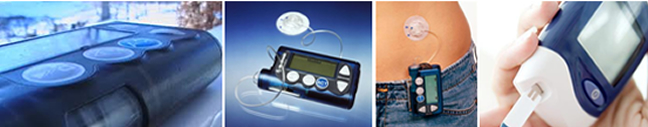
\includegraphics[scale=1]{images/bombainsulina.png}
	\caption{Imagens de uma bomba de infusão de insulina}	
	\label{fig:bombainfusao}	
\end{figure}


Seu funcionamento é bem simples, libera-se uma quantidade de insulina, programada pelo médico, durante o dia todo, simulando o funcionamento do pâncreas de uma pessoa saudável, entretanto existem cuidados a serem tomados: calcular a quantidade de carboidratos ingeridos a cada refeição e programar o aparelho para injetar uma quantidade de insulina com maior velocidade no organismo nos horário em que se faz as refeições principais.
Quanto a quem pode usar, a pessoa deve cumprir alguns pré-requisitos que são:
\begin{itemize}
\item Conseguir medir o índice glicêmico no mínimo 4 vezes por dia;
\item Durante a fase de adaptação e ajuste da dosagem a serem utilizadas pela bomba, fazer a medição glicêmica de 6 a 8 vezes por dia;
\item Seguir as recomendações médicas além de manter contato e um constante \emph{feedback} com os responsáveis pela bomba e, além de tudo, seguir a dieta recomendada, respeitando quantidades ingeridas;
\item Ter condição financeira para custear o equipamento e o contato com os responsáveis por ele;
\item Estar disposto ao uso da bomba durante o dia todo, 24 horas junto ao corpo;
\item Aprender sobre contagem de carboidratos para saber seu consumo durante as refeições;
\item Praticar exercícios.
\end{itemize}

Cumprindo os pré-requisitos citados temos as vantagens de seu uso que são:

\begin{itemize}
\item Maior flexibilidade no horário das refeições;
\item Se usada corretamente o risco de hipoglicemia é reduzido, e a longo prazo as complicações devido ao diabetes também;
\item Melhora o controle glicêmico;
\item Melhora no controle do fenômeno do amanhecer, responsável pelo aumento do índice glicêmico durante a manha, entre as 4 e 8 horas da manha, causador da hipoglicemia se o diabético não calculou a dose de insulina antes de dormir, ou não se levantou durante a noite para gerenciá-la.
\end{itemize}

Mas mesmo com todas as vantagens dada devido ao uso do equipamento caso o diabético seja obeso, ingira grandes quantidades de alimento ou açúcar, ou seja, carboidratos, não praticar atividades físicas, não fazer a medição do índice glicêmico na quantidade de vezes recomendada, ou até mesmo determinar por si só a quantidade de insulina a ser utilizada, não existe vantagem no seu uso.
É importante ter em mente que mesmo com toda facilidade e tecnologia existente o acompanhamento médico não deve ser deixado de lado. As principais indicações médicas para o uso do equipamento são:

\begin{itemize}
\item Fenômeno do amanhecer;
\item Hipoglicemia;
\item Diminuir a variação do índice glicêmico;
\item Hiperglicemia;
\item Recorrente ceatosidade, que é o acumulo de ceatócidos, pois o fígado quebra a gordura e proteína devido à falta de insulina, pois o corpo não consegue utilizar a glicose como energia;
\item Flexibilidade, especialmente para crianças pequenas;
\item Gestação, viagens e atividade físicas;
\item Fobia de injeção;
\item Desejo do diabético \cite{diabetes2013, portaldiabetes2009}.
\end{itemize}

\section{Motivação}
Segundo a Sociedade Brasileira de Diabetes \cite{sbc2014}, diversos estudos realizados mostram que o tratamento feito através da Infusão de insulina tem diversas melhorias quando comparado com outros tratamentos existentes. Entretanto não é o mais utilizado devido ao seu alto custo, devido a importação.
Logo, esse projeto vem com foco social: facilitar o acesso da população brasileira de baixa renda ao equipamento, melhorando sua qualidade de vida dos portadores da doença que se encaixem nesse perfil. 

\section{OBJETIVOS}
Esse projeto tem como objetivo principal desenvolver um software para um protótipo de uma Bomba de Infusão de insulina utilizando o microcontrolador da família PIC, PIC18F452. 

\subsection{OBJETIVOS SECUNDÁRIOS}

Em segundo plano este trabalho foca em:
\begin{itemize}
\item Aprendizado sobre as características e funcionalidades disponíveis do microcontrolador escolhido;
\item Aprendizado das tecnologias utilizadas como: compilador, simulador e bibliotecas disponíveis;
\item Desenvolvimento das funcionalidades básicas de uma bomba de infusão de insulina;
\item Aprendizado sobre a escolha e uso de um motor de passo;
\item Aprendizado sobre a forma de uso de um \emph{display} de LCD para comunicação com o usuário.
\end{itemize}

\section{PROCEDIMENTOS METODOLÓGICOS}
Este trabalho foi dividido em duas etapas: pesquisa para levantamento de referências bibliográficas e desenvolvimento prático. Durante a primeira etapa, foi feita a pesquisa e levantamento bibliográfico sobre o tema em questão para que fosse possível um melhor entendimento da plataforma, tecnologias e, claro, do problema abordado. Juntamente com essa pesquisa, foi feito um estudo sobre o microcontrolador PIC escolhido, PIC18F452, a partir do material encontrado. O estudo e desenvolvimento foi feito utilizando o compilador MikroC e sua IDE, já para os testes utilizou-se o simulador Proteus. Em seguida houve-se um levantamento de informações sobre sistemas embarcados, sistemas críticos e sistemas críticos de tempo real, e assim adquirindo-se conhecimento sobre os conceitos de desenvolvimento da área em questão, uma vez que a confiabilidade e segurança do problema proposto é importantíssimo.


O software de controle do protótipo da bomba de infusão de insulina foi desenvolvido na linguagem C, compilado para o microcontrolador já citado, PIC18F452. O sistema é responsável basicamente por gerenciar o perfil de infusão basal, calcular intervalos corretos e passos necessários para uma infusão. Desta forma, o
software foi dividido nos seguintes módulos: Config, LCD, InsulinPump, Motor, Menu, TimerMotor e principal. 

Essa divisão por módulos é, e foi, extremamente importante para o desenvolvimento do sistema. Somando-a à um dos conceitos mais importante desse projeto - OOC, \emph{Object-Oriented Programming With ANSI-C} - são as chaves para a facilidade de manutenção, entendimento do código e possível evolução do projeto.

As responsabilidade dos módulos são bem claras e isoladas:

Config: Centralizar configurações gerais do sistema;
LCD: Abstrair uso do periférico para o resto do sistema;
InsulimPump: Abstrair funcionamento, requisitos de segurança e outras particularidades da bomba;
Motor: Abstrai como se controla o motor e qual tipo está sendo utilizado para infusão;
TimerMotor: Separa o gerenciador de tempo das particularidade únicas do hardware e compilador;
Menu: Facilitar navegação entre menus, simulando máquina de estado;
Principal: Possui o \emph{loop} principal para navegação simples entre os menus existentes.

E, finalizando, após o desenvolvimento, executou-se uma bateria de testes para se o funcionamento da bomba estava sendo de acordo coma forma especificada, levando em conta toda a integração necessária com os periféricos existentes.


% ----------------------------------------------------------
% Sistemas Embarcados
% ----------------------------------------------------------
\chapter{SISTEMAS EMBARCADOS}
Sistema embarcado em geral é uma combinação de \emph{hardware} e \emph{software} para executar uma tarefa específica diferente dos computadores do dia-a-dia que possuem inúmeros propósitos: verifica e-mail, escrever monografias, entre outros. Sistemas embarcados podem possuir ou não um sistema operacional, seja um RTOS, possui requisitos de tempo de execução, ou um Linux e, portanto, pode ser desenvolvido em um \emph{hardware} com microcontrolador ou microprocessador \cite{wikibook2012embedded}.

Segundo \cite{cunha2013} a inteligência embarcada é uma tendência futura, cada vez mais inteligência será adicionada aos equipamentos do dia-a-dia, considera que um micro-ondas atual tem mais capacidade computacional do que tinha o projeto Apolo, que levou o homem a lua. Esta crescente utilização se dá basicamente pelo preço e consumo reduzido dos microcontroladores, além da grande flexibilidade ao atender os mais diversos problemas visto o vasto número de arquiteturas disponíveis: ARM, MIPS, Coldfire/68k, PowerPC, x86, PIC, 8051, Atmel AVR, Renesas H8, SH, V850, FR-V, M32R, Z80, Z8 e outras. Um contraste que atrai diversos desenvolvedores quando comparado com o número limitado de arquiteturas diponíveis para microprocessadores do mercado de computadores pessoais \cite{germano2011}.

A comunicação dos microcontroladores com o meio externo, segundo \cite{germano2011}, se dá pelos periféricos e o mais comuns são:
\begin{itemize}
\item Entrada de dados através de teclas, geralmente pelo de teclados feitos com varredura matricial;
\item \emph{Leds};
\item \emph{Display’s} de LCD, sendo os mais comuns os alfanuméricos como o HD44780;
\item Interface serial, por exemplo RS232 e I2C;
\item USB, \emph{Universal Serial Bus};
\item TCP/IP.
\end{itemize}

Como dito anteriormente, esses sistemas estão cada vez mais no dia-a-dia das pessoas e, claro, facilitando a vida delas, mas muitas vezes não são percebidos. E cada vez mais estão mais acessíveis podendo automatizar funções até mesmo dentro das próprias casas. A Figura \ref{fig:exemplosistemasembarcados}\footnote{\url{http://bytesdontbite.com/2012/06/26/embedded-systems-no-bdb/}} mostra alguns sistemas embarcados e onde são utilizados:

\begin{figure}[htp]
	\centering
	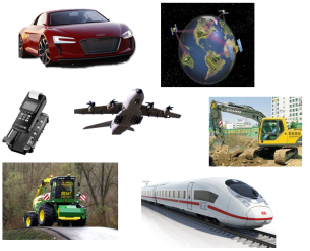
\includegraphics[scale=1]{images/exemplo_sistemas_embarcados.png}
	\caption{Exemplo de Sistemas embarcados}	
	\label{fig:exemplosistemasembarcados}	
\end{figure}

\section{SISTEMAS EMBARCADOS DE TEMPO}
O conceito Tempo Real é complexo para ser explicado, mas sua ideia básica é que se espera que o computador responda algo para o ambiente externo em tempo. Normalmente pessoas assumem que tempo real significa "muito rápido", entretanto não é verdade, tempo real simplesmente significa "rápido o suficiente" no contexto de operação do sistema. Um exemplo é a ação do motor, pode-se dizer que é "rápida", pois o sistema deve tomar decisões como - fluxo de combustível, tempo da faísca - toda vez que o motor completa um ciclo.

Sistemas de tempo real são baseados em previsibilidade e, segundo \cite{farines2000sistemas}, essa previsibilidade de um sistema de tempo real é obtida quando independente de falhas, sobrecargas e variações de hardware, e assim é possível que seu comportamento seja antecipado antes de sua execução. Isso tem a finalidade de poder prever o funcionamento de um sistema de tempo real e garantir as suas restrições temporais, e para isso é necessário definir hipóteses em relação a carga e falhas em relação ao ambiente externo deste sistema \cite{farines2000sistemas}. 
Segundo \cite{mall2009real} os sistemas de tempo real são classificados em dois tipos:
\begin{itemize}
\item \emph{Soft Real Time Systems}: Sistemas não críticos de tempo real, onde a ocorrência de uma falha temporal é da mesma ordem de grandeza que os resultados em que o funcionamento está correto, exemplos: Máquina de lavar e portão eletrônico de uma casa;
\item \emph{Hard Real Time Systems}: Sistemas Críticos de Tempo Real, onde a ocorrência de uma falha temporal complicam, e muito, os resultados quando comparado com seu funcionamento correto, exemplos: sistema de controle de um avião e um sistema de controle de semáforos.
\end{itemize}

\section{SISTEMAS EMBARCADOS CRÍTICO}
\label{sec:SistemaEmbarcado}

Sistema Crítico é um sistema no qual a confiança é fundamental, ou melhor, a questão mais importante em seu desenvolvimento. Isso porque sistemas críticos, em caso de falha, podem causar consequências gravíssimas para os humanos, economia e outras áreas. Pode-se dizer que seus indicadores são: Disponibilidade, confiabilidade, segurança e proteção. E para que essa confiança seja alcançada deve-se evitar erros durante seu desenvolvimento e realizar diversos testes para que seja possível detectar e corrigir os erros que passarem de forma que seja possível limitar os danos causados por falhar operacionais \cite{sommerville2004software,feldmann2007survey,jordan2006standard}.

Segundo \cite{kopetz2011real} as classificações dos sistemas embarcados críticos podem ser:
\begin{itemize}
\item \emph{Fail Safe}: Classificação para sistemas onde o estado seguro pode ser atingido em caso de falha, como por exemplo, esgotar a bateria de uma bomba de insulina;
\item \emph{Fail Operational}: Classificação para sistemas que em caso de falhas ainda são capazes de fornecer algum tipo de serviço, mesmo que mínimo. Um exemplo é um sistema de controle de voo que, mesmo em caso de falha, é capaz de fornecer serviços e ser seguro.
\end{itemize}

Abaixo a Figura \ref{fig:exSistEmbarcado},  mostra exemplos de sistemas embarcados críticos.

\begin{figure}[htp]
	\centering
	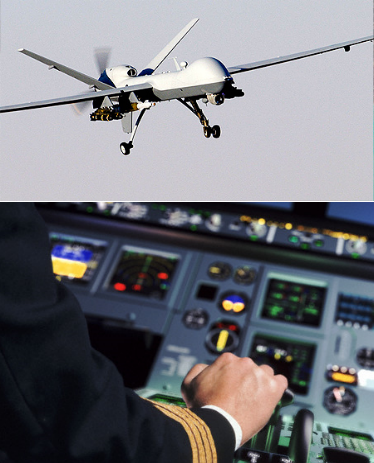
\includegraphics[scale=0.7]{images/exemplo_sistemas_embarcados_criticos.png}	
	\caption{Sistemas embarcados críticos}
	\label{fig:exSistEmbarcado}	
\end{figure}

\section{MICROCONTROLADOR}
Microcontroladores são chips inteligentes que utilizam a arquitetura Harvard, RISC. É constituído basicamente por pinos de entradas e saídas e memória. Suas saídas podem ser controladas através de programação e em função do processamento de suas entradas. Sua programação pode ser feita em diversas linguagens como: C, C++, entre outras \cite{radio2012amadores}.

Segundo \cite{ganssle1999art}, o microcontrolador é a parte mais importante de um sistema embarcado e sua principal diferença quando comparada com um microprocessador é o fato de ser um sistema computacional completo que integra todos as principais partes da arquitetura de Von Neumann em um único componente, as partes citadas são:
\begin{itemize}
\item CPU: \emph{Central Processor Unit};
\item Memória RAM: \emph{Random Access Memory};
\item Portas I/O: Portas de entrada e saída.
\end{itemize}

Além de ser composto por temporizadores, memória ROM (\emph{Read Only Memory}), conversor AD, analógico – digital, e DA, digital – analógico.
Comparados com microprocessadores, os microcotroladores possuem consumo e \emph{clock}, processamento, reduzidos, isso devido ao fato que o primeiro é destinado a tarefas que necessita uma alta capacidade de processamento como, por exemplo, os microprocessadores do nosso PC do dia-a-dia. Por padrão, os microprocessadores são utilizados em situações que os requisitos são abrangentes, com entradas e saída variadas como: sensores, atuadores e periféricos de comunicação \cite{lee2011introduction}.

\subsection{PIC}
PIC é um circuito integrado produzido pela \emph{Microchip Technology Inc}. Seu nome significa: \emph{Programmable Interface Controller}, Controlador de Interface Programável. Externamente possui uma aparência de um circuito integrado mais comuns - TTL ou CMOS -, mas na verdade contém todos os componentes de um sistema microprocessado como: CPU, \emph{Central Processor Unit}, sua finalidade é interpretar as instruções de programa; Memória PROM, \emph{Programmable Read Only Memory}, na qual memorizará as instruções do programa; Memória RAM, \emph{Random Access Memory}, utilizada pra memorizar as variáveis do programa; Linhas de I/O, entrada e saída, para controlar dispositivos internos e receber informações do meio externo; entre outros \cite{radio2012amadores,wikipedia2012pic}.

\subsection{SENSORES}
A definição de sensor pode ser a de um transdutor capaz de alterar sua característica física interna em resposta à um fenômeno físico externo. Além disso, existem sensores considerados de operação indireta que são os quais alteram suas propriedades como capacitância, resistência, ou, até mesmo, sua indutância, sob ação de algum gradeza ou evento externo \cite{rosario2006principios}. 

Segundo \cite{nomadusp2014}, os sensores são largamente utilizados na medicina, indústria, robótica, além de outras aplicações. Considerando que o sinal é sempre uma forma de energia, os sensores podem ser classificados em função da energia que é capaz de detectar, como:

\begin{itemize}
\item Sensores de luz: células solares, fotodíodos, fototransistores, tubos fotoelétricos, e outros;
\item Sensores de som: microfones e hidrofone;
\item Sensores de temperatura: termômetros e termopares;
\item Sensores de resistência elétricas: ohmímetro. 
\item Outros;
\end{itemize}

\subsection{SENSORES BIOLÓGICOS}
Segundo \cite{nomadusp2014}, os sensores citados anteriormente são corretamente chamados de sensores artificiais. Isto devido ao fato de existir sensores naturais ou biológicos, já que todos os organismos vivos possuem sensores capazes de agir da mesma forma que os artificias. Esses sensores biológicos são células especializadas, sensíveis a:

\begin{itemize}
\item Luz, movimento, temperatura, vibração, pressão, campos eléctricos, som, e outros aspectos físicos do ambiente;
\item Grande variedade de moléculas ambientais, incluindo toxinas e nutrientes;
\item Aspectos metabólicos, tais como os níveis de glicose e oxigênio;
\item Até mesmo as diferenças entre proteínas do ambiente externo e do próprio organismo.
\end{itemize}

Esses sensores artificiais que imitam sensores biológicos, utilizando componentes biológicos, são chamados biossensores.

\subsection{ATUADORES}
Segundo \cite{chironis1991mechanisms}, dispositivos considerados atuadores são aqueles que transformam uma forma de energia em outra, causando mudanças no ambiente em que estão atuando, ou seja, de acordo com sinais, ou impulsos, recebidos realizam ações capazes de alterar as grandezas físicas do ambiente em questão. Eles são capazes de converter energias como: energia elétrica, hidráulica e pneumática em energia mecânica. Segue exemplos de alguns tipos de atuadores:

\begin{itemize}
\item Atuadores eletromagnéticos: São os motores elétricos como motores de passos, servos;
\item Atuadores hidráulicos: Utilizam um fluido submetido a uma pressão para movimentar um braço, são utilizados em robô que operam grandes cargas;
\item Atuadores pneumáticos: Utilizam um gás submetido a uma pressão para movimentar o braço, possuem menor custo que os hidráulicos, sendo utilizados em robôs de menor porte;
\end{itemize}

\subsection{MOTOR DE PASSO}
Motor de passo é um dispositivo eletromecânico. Sua principal propriedade é sua habilidade de transformar pulsos elétricos em movimentos, que são precisamente incrementados na posição do rotor e são denominados "passos". Esse tipo de motor é caracterizado como máquina duplamente saliente, significando que possui dentes, compostos por matérias magnéticos nas duas partes que o compõe: A parte imóvel chamada estator e a móvel rotor \cite{demotor, acarnley2002stepping}.

Seu uso é interessante em situações em que precisão nos movimentos é necessária. Isso porque com ele é possível controlar: ângulo de rotação, velocidade, posição e sincronismo. Suas vantagens não são seu torque nem a capacidade de gerar movimentos de alta velocidade, mas sim a precisão em seus movimentos. Devido a essas características esse tipo de motor é amplamente utilizado em: câmeras de vídeo, robôs, brinquedos, \emph{scanners}, impressoras, entre outros \cite{demotor}.

De forma simples o funcionamento de um motor de passo consiste no uso de materiais magnéticos, ou solenoides, como dito anteriormente, alinhados dois a dois, representando os polos norte e sul, que quando energizados atraem o rotor fazendo-o se alinhar as partes energizadas do estator, causando assim um pequeno movimento: o passo. Sua velocidade e sentido estão diretamente relacionados à forma com que os solenoides são acionados, o primeiro com a frequência e o segundo a ordem de acionamento \cite{demotor, acarnley2002stepping,wikipedia2012stepper}.

\subsection{MOTOR DE PASSO RELUTÂNCIA VARIÁVEL – \emph{MULTI STACK}}
A fonte do fluxo magnético desse tipo de motor são as bobinas colocadas nos dentes do estator. O acionamento das bobinas é feito em sequência para incentivar o movimento, alinhamento, dos conjuntos de dentes sucessivos do estator e do rotor dando ao motor a característica de passos. Ao longo de eu eixo ele é dividido em seções isoladas magneticamente chamadas \emph{stacks}, daí o nome \emph{multi stack}, e cada uma pode ser excitada por uma bobina separadamente chamada phase. Cada \emph{stack} possui um estator, preso em sua posição pela caixa, suporte, do motor junto com as bobinas e o elemento móvel, rotor.

O rotor é uma unidade única e maciça que será utilizado para a movimentação da carga. O material do rotor é um metal elétrico laminado o que permite que o campo magnético possa mudar rapidamente sem grandes perdas. O estator de cada rotor possui um determinado número de polos e uma parte da \emph{phase}, bobina, é enrolada em torno de cada polo para produzir o campo magnético. Os polos adjacentes são enrolados no sentido oposto assim os campos magnéticos adjacentes possuem sentidos opostos. Com isso o circuito magnético completo é considerado um polo do estator, o dente do rotor, o vão de ar entre os dentes de ambos e, por fim, um polo adjacente do estator. E esse circuito é repetido a cada par de polos do estator. As forças normais produzidas pelos polos do estator e os dentes do rotor são iguais e se anulam assim sobra apenas a força tangencial o que causa o movimento, isso pode ser visto conforme a Figura ~\ref{fig:forcamotorpassobainfusao}.

\begin{figure}[htp]
	\centering
	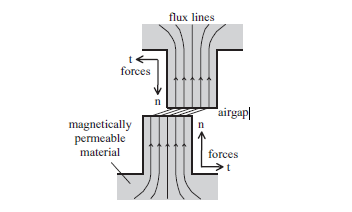
\includegraphics[scale=1]{images/forca_motor_passo.png}
	\caption{Forças normais e tangenciais}	
	\label{fig:forcamotorpassobainfusao}	
\end{figure}

A posição do rotor com relação ao estator é ajustada toda vez que as bobinas são excitadas. O ajuste ocorre, pois os dentes de ambos são alinhados o que tende a diminuir a relutância do circuito magnético, daí surgiu o nome do motor. Considerando a Figura ~\ref{fig:visaomotorpasso} é possível perceber que para girar no sentido horário a ordem de acionamento deve ser A, B, C, A, B, C, A... e no sentido anti-horário A, C, B, A, C, B, A...

\begin{figure}[htp]
	\centering
	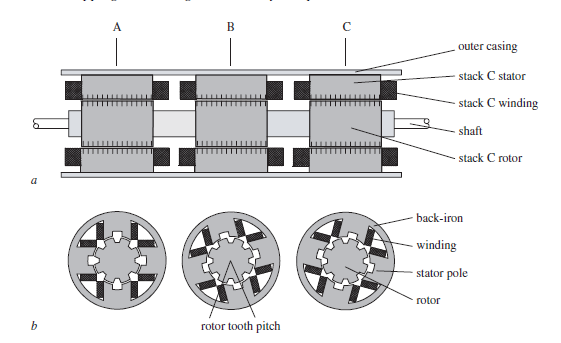
\includegraphics[scale=1]{images/visao_motor_passo.png}
	\caption{Visão paralela e perpendicular das \emph{stacks} e rotor}	
	\label{fig:visaomotorpasso}	
\end{figure}

\newpage Segundo \cite{acarnley2002stepping}, existe uma pequena relação entre o comprimento do passo. Considere N o número de dentes do estator e p o número de dentes do rotor logo: 

\begin{equation}
  \emph{step length} = 360/(N * p)
\end{equation}

\subsubsection{\emph{DESIGN} DO MOTOR}
Cada polo do estator produz um campo magnético quando excitado com uma corrente DC. A performance do motor depende da força do campo magnético gerado pelas bobinas quando excitadas, logo o campo magnético está diretamente ligado ao torque do motor. A força do campo magnético está relacionada à intensidade da corrente que passa pelas bobinas, portanto em teoria aumentar a corrente para aumentar o torque seria o suficiente, entretanto existe um limitante que é o aumento da temperatura nas bobinas.

No exemplo da Figura ~\ref{fig:visaomotorpasso} cada \emph{stack} tem 4 polos. Uma vez que todas as quatro bobinas devem ser excitadas concorrentemente uma prática comum é interconectar as bobinas para formar apenas uma \emph{phase}. A forma com que as bobinas são interconectadas influência na temperatura que será dissipada pela bobina uma vez que isso está diretamente ligada à intensidade da corrente. A potência não varia conforme a interconexão. 

Existem 3 formas de interconexão conforme a Figura ~\ref{fig:bobinas}. Na verdade a potência não varia conforme a interconexão, mas sim qual \emph{driver} de controle será utilizado: baixa voltagem e alta corrente com uma conexão paralela ou alta voltagem e baixa corrente com uma conexão em série. A diferença entre as 3 interconexões pode ser vista na Figura ~\ref{fig:relacaobobina} \cite{acarnley2002stepping}.

\begin{figure}[htp]
	\centering
	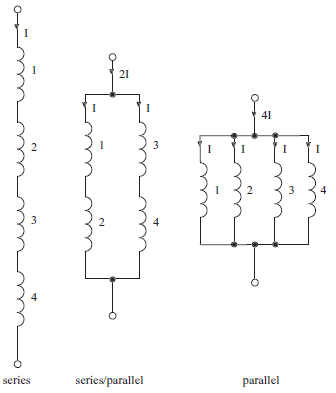
\includegraphics[scale=1]{images/bobinas.png}
	\caption{Interconexão das bobinas}	
	\label{fig:bobinas}	
\end{figure}

\begin{figure}[htp]
	\centering
	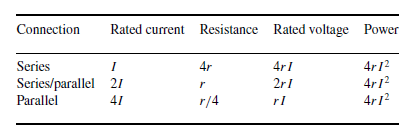
\includegraphics[scale=1]{images/relacao_bobina.png}
	\caption{Relação das interconexões das bobinas}	
	\label{fig:relacaobobina}	
\end{figure}

\subsection{MOTOR DE PASSO RELUTÂNCIA VARIÁVEL – \emph{SINGLE STACK}}
Como o nome já diz esse motor é construído com apenas uma stack, ou melhor, uma unidade. Entretanto quanto ao funcionamento e princípios básicos é idêntico ao \emph{multi stack}. Cada dente do estator ainda possui uma bobina separada que produz um campo magnético quando excitada por uma corrente DC.

Uma mudança é que as bobinas do lado oposto são conectadas para formar uma phase. Na Figura ~\ref{fig:singlestack} existe 3 phases que é o número mínimo para poder rotacionar para os dois lados. A bobina no dente oposto no estator está no sentido oposto para que sejam gerados campos magnéticos em sentidos opostos. E por fim a relação de comprimento do passo se mantém conforma o motor \emph{multi stack} \cite{acarnley2002stepping}.

\begin{figure}[htp]
	\centering
	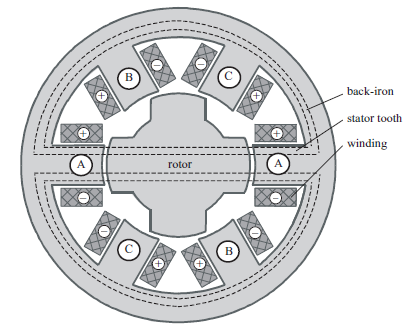
\includegraphics[scale=1]{images/single_stack.png}
	\caption{\emph{Stator single stack}}	
	\label{fig:singlestack}	
\end{figure}

\subsection{MOTOR DE PASSO HÍBRIDO}
A diferença principal desse com os tipos anteriores é que o circuito magnético é excitado por uma combinação de bobinas e imã permanente. Seu funcionamento e princípios básicos são idênticos ao \emph{multi} e \emph{single stack}. As bobinas ainda permanecem nos dentes do estator já o imã compõe o eixo do rotor conforme Figura ~\ref{fig:hibrido}.

\begin{figure}[htp]
	\centering
	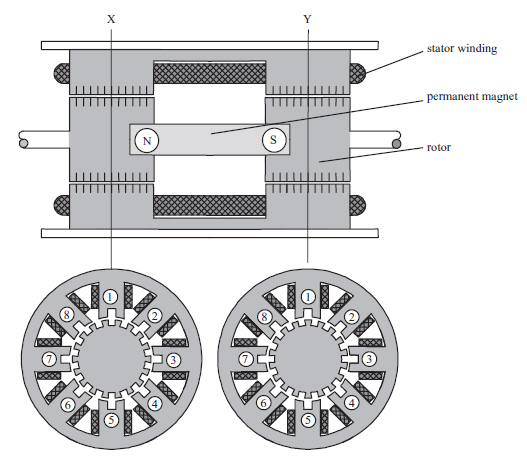
\includegraphics[scale=0.7]{images/hibrido.png}
	\caption{Motor híbrido}	
	\label{fig:hibrido}	
\end{figure}

Existem duas bobinas, \emph{phases}, situadas em 4 dos 8 polos do estator, conforme Figura \ref{fig:hibrido}. A bobina A está nos polos 1, 3, 5, 7 e a B nos polos 2, 4, 6, 8. Polos adjacentes ainda são envolvidos pelas bobinas em sentidos opostos, portanto se a bobina A é alimentada com corrente positiva o campo magnético é direcionado para fora nas bobinas 3 e 7, mas para dentro nos polos 1 e 5 e o mesmo acontece na bobina B.

Quando se aplica corrente nas bobinas a mesma ideia de alinhamento dos dentes do rotor e stator acontece. Considerando a Figura \ref{fig:hibrido} e o exemplo da excitação positiva na bobina A, citada anteriormente, o estator e o rotor são alinhados sob os polos 3 e 7 na seção X e polos 1 e 4 na seção Y.

Para uma rotação continua o motor necessita de uma excitação sequencial das bobinas. Se retirar a excitação de A e colocar em B o alinhamento dos dentes vai acontecer com 4 e 8 na seção X e 2 e 6 na seção Y. Isso faz com que o motor gire no sentido horário, a sequência deve ser A+, B+, A-, B-,... Para o sentido anti-horário A+, B-, A-, B+.

Segundo \cite{acarnley2002stepping}, a relação de comprimento do passo é similar ao de relutância variável. Existe uma relação com o número de dentes do rotor p, e com um ciclo completo de excitação. Como um esse ciclo em um motor hibrido consiste em 4 estados e produz 4 passos de movimento no rotor, logo conclui-se que:
\begin{equation}
  \emph{step length} = 360/(4 * p) = 90 / p
\end{equation}

\subsection{COMPARAÇÃO ENTRE TIPOS DE MOTORES}
Não é possível dizer categoricamente que um motor é melhor do que o outro em todas as situações. Os híbridos têm menor comprimento de passo, normalmente 1,8 graus, o que pode ser uma grande vantagem quando alta precisão é necessária. Eles também possuem maior torque devido ao uso do imã permanente no rotor. E, além disso, quando nenhuma bobina esta excitada o motor hibrido ainda possui um "torque de retenção" que mantém a posição do rotor. E isso pode ser uma característica na aplicação onde a posição do rotor deve ser preservada durante uma falha de energia, mas é bom lembra que esse torque é menor do que o torque com 1 ou mais bobinas excitadas.

Já o de relutância variável tem duas vantagens quando se trata de movimentar carga em distâncias consideráveis. A primeira é que tipicamente o comprimento de seu passo é de 15 graus, maior que o do híbrido, portanto ele precisa de menos passos para mover a mesma distância. Com a redução do número de excitações das bobinas o consumo também é reduzido, em caso de uso de baterias é uma característica muito interessante. A segunda é que por não possuir imã permanente possui uma menor inércia para início de movimento, também diminuindo o consumo inicial \cite{acarnley2002stepping}.

\subsection{LCD - \emph{Liquid Crystal Display}}
Um \emph{display} de cristal líquido, LCD, é utilizado para exibir informações como texto, imagens e vídeos. É composto por um painel fino e, segundo \cite{lcd1996unicamp}, é um componente, considerado interface de saída, muito utilizados em conjunto com microcontroladores. Exemplos de uso são: \emph{cockpit} de aeronaves, \emph{displays} em computadores de bordo de automóveis, dispositivos de jogos, relógios, calculadoras e outros.

Pode-se classificar os módulos de LCD em: exibição gráfica e exibição de caractere. Os módulos gráficos são encontrados com resoluções de 122x32, 128x64, 240x64 e 240x128 pixel, possuindo, geralmente, 20 pinos para conexão. Já os modelos comuns, tipo caractere, tem sua especificação em função dos números de linhas e colunas, a Figura \ref{fig:pinoslcd} representa seus sexemplos.

\begin{figure}[htp]
	\centering
	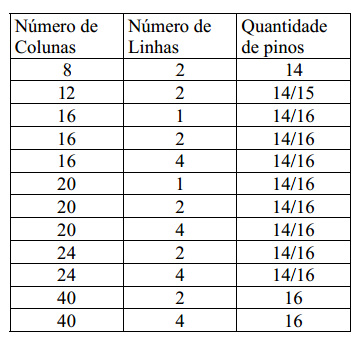
\includegraphics[scale=1]{images/tabelas_pinos_lcd.png}
	\caption{Tabelas de pinos LCD comum}	
	\label{fig:pinoslcd}	
\end{figure}

% ----------------------------------------------------------
% Proteus
% ----------------------------------------------------------
\chapter{PROTEUS \emph{DESIGN SUITE}}
Proteus é um suíte, conjunto de \emph{features}, desenvolvido pela Labcenter Eletronics Ltd. É um software para: simulação de microcontroladores, simulação de circuitos eletrônicos e para desenvolvimento de placa de circuito impresso. Os componentes desse sistema são:
\begin{itemize}
\item ISIS \emph{Schematic Capture}: Ferramenta utilizada para se adicionar objetos, componentes para simulação;
\item PROSPICE \emph{Mixed mode SPICE simulation}: Simulador industrial padrão SPICE3F5, combinado com simulador digital de alta velocidade. \emph{Spice, Simulation Program with Integrated Circuit Emphasis}, é um simulador para propósitos gerais para sistemas eletrônicos analógicos.
\item ARES PCB \emph{Layout}: Sistema de PCB, \emph{Printed Circuit Board}, ou melhor, placa de circuito impresso, design de alto desempenho com posicionamento automático de componente, auto-roteamento, entre outras \emph{features} relacionadas ao desenvolvimento de placas de circuito impresso.
\item VSM - \emph{Virtual System Modelling}: Permite simular software embarcado para microcontroladores, disponíveis em suas bibliotecas, ao lado de seu projeto de hardware \cite{proteus2013, wikipedia2012spice}.
\end{itemize}

\section{ISIS \emph{SCHEMATIC CAPTURE}}
Como já foi dito, essa feature se trata da funcionalidade de simulação e montagem de circuitos eletrônicos. Permite que o circuito em questão seja debugado de forma simples e, além disso, possibilita uma integração com códigos desenvolvidos para microcontroladores suportados por ele. Seus componentes são:

\begin{itemize}
\item Circuitos integrados das famílias: 74ALS, 74AS, 74F, 74HC, 74HCT, 74LS, 74S e 74STD;
\item Componentes analógicos;
\item Medidores de corrente e tensão para serem utilizados durante o debug;
\item Geradores como fontes e clock, ambos ajustáveis para o valor desejado;
\item Semicondutores como diodo, transistor, LEDs e outros;
\item Componentes básicos como chaves, resistores, capacitores e indutores;
\item Atuadores como motor DC, motor de passo e outros;
\item Microcontroladores da família 80XXX, AT e PIC;
\item Memórias, displays, CMOS e outros.
\end{itemize}

Seu uso é bem simples, pois é como se estivesse desenhando o circuito em um papel. Após ser desenhado é possível utilizar as ferramentas de auxilio para debug e assim coletar dados como voltagem e corrente do circuito e até mesmo se o funcionamento está conforme o esperado.

% ----------------------------------------------------------
% MikroC
% ----------------------------------------------------------
\section{MIKROC}
MikroC é um \emph{toolchain} poderoso, uma ferramenta de desenvolvimento completa para microcontroladores da família PIC. Criado de forma que disponibilize ao usuário a forma mais fácil de desenvolver suas aplicações para sistemas embarcados, sem compromisso de desempenho ou controle. MikroC permite que seja feito um rápido desenvolvimento e embarcar aplicações complexas:

\begin{itemize}
\item Escrever códigos em C utilizando um editor de código avançado;
\item Utilizar as bibliotecas do próprio MikroC para acelerar o desenvolvimento: aquisição de dados, memória, \emph{display}, comunicação, entre outros;
\item Auxilia na evolução e desenvolvimento do código monitorando a estrutura do programa, variáveis e funções. Gera um código comentado, humanamente legível em assembler, e um padrão HEX compatível com o padrão conhecido;
\item Possui um \emph{debugger} integrado capaz de gerar relatórios detalhados, estatísticas, pilha de execução, entre outras opções que auxiliam analisar o fluxo do programa \cite{mikroc2006}.
\end{itemize}

% ----------------------------------------------------------
% PIC18F452
% ----------------------------------------------------------
\section{PIC18F452}
O PIC18F452 é um microcontrolador fabricado pela empresa \emph{Microchip Technology}. Possui tecnologia CMOS, como consequência tem um consumo baixíssimo, possui memória do tipo FLASH, um grande facilidade para desenvolvimento de protótipos, uma vez que para apagá-la não é preciso utilizar luz ultravioleta como em versões antigas, utilizavam memória EEPROM. Abaixo seguem as principais características desse microcontrolador:

\begin{itemize}
\item Microcontrolador de 40 Pinos;
\item Memória de programa FLASH de 32Kbytes;
\item Memória RAM de 1536 bytes;
\item Memória EEPROM de 256 bytes;
\item Processamento de até 10MIPS;
\item Quatro \emph{timers}, ou temporizadores, internos – um de 8 bits e 3 de 16 bits – TIMER0, TIMER1, TIMER2 e TIMER3;
\item 2 canais capture/compare/PWM – Módulo CCP;
\item Módulo \emph{Master Synchronous Serial Port} (MSSP);
\item \emph{Unhaced Usart;}
\item 8 canais A/D de 10 bits;
\item Detector de baixa voltagem programável;
\item Permite até 100.000 ciclos de escrita e leitura na memória FLASH;
\item Permite 1.000.000 ciclos de escrita e leitura na memória EEPROM.
\item Retenção de dados na FLASH por 40 anos;
\item \emph{Watchdog timer} com oscilador próprio e programável;
\item Três pinos de interrupções externas: INT0, INT1 e INT2
\end{itemize}

A Figura \ref{fig:pic} representa uma imagem do microcontrolador.

\begin{figure}[htp]
	\centering
	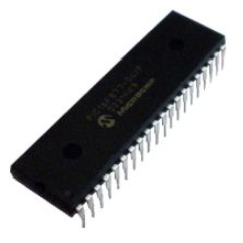
\includegraphics[scale=1]{images/pic.png}
	\caption{PIC18F452}	
	\label{fig:pic}	
\end{figure}

\newpage 
\subsection{Estrutura Interna}
A Figura \ref{fig:estuturapic} ilustra como é a estrutura interna do microcontrolador:

\begin{figure}[htp]
	\centering
	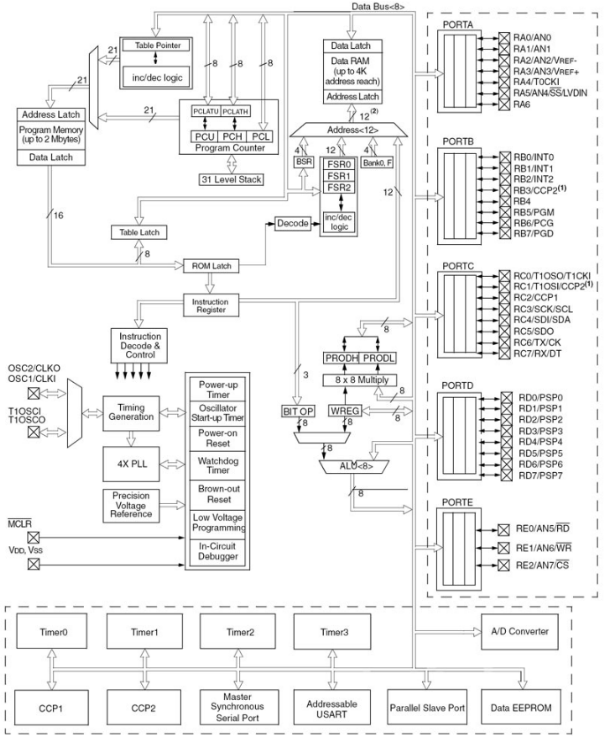
\includegraphics[scale=0.6]{images/estrutura_pic.png}
	\caption{Estrutura Interna PIC18F452}	
	\label{fig:estuturapic}	
\end{figure}

\newpage 
\subsection{DESCRIÇÃO DOS PINOS}
Dos 40 pinos desse microcontrolador 34 são pinos I/O, entrada e saída, divididos em 5 "PORT". A Figura \ref{fig:pinospic} representa uma relação dos pinos do microcontrolador.

\begin{figure}[htp]
	\centering
	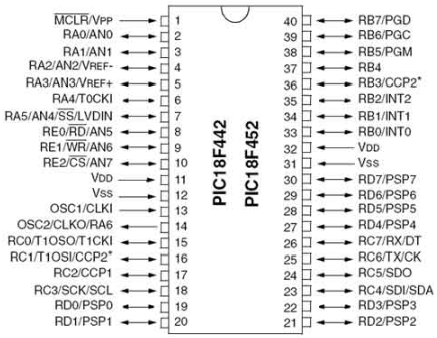
\includegraphics[scale=0.6]{images/pinos_pic.png}
	\caption{Pinos PIC18F452}	
	\label{fig:pinospic}	
\end{figure}

A divisão dos pinos I/O citada é da seguinte maneira:

\begin{itemize}
\item PORTA: São 7 pinos nomeados de RA0 a RA6. Podem ser utilizados como I/O geral ou conversor A/D, essa segundo opção tem exceção o pino RA4. Além de possuir a opção LVD, detecção de baixa tensão;
\item PORTB: São 8 pinos nomeados de RB0 a RB7. Podem ser utilizados para I/O geral e, além disso, pode-se trabalhar com três interrupções externas, módulo CCP, pinos de gravação e debug;
\item PORTC: São 8 pinos nomeados de RC0 a RC7. Podem ser utilizados para I/O geral, saída do oscilador do \emph{timer}, módulo CCP, Clock e data(dados) para os modos SPI, I2C e UART;
\item PORTD: São 8 pinos nomeados de RD0 a RD7. Podem ser utilizados para I/O geral ou como PSP para ter saída TTL, para interfaceamento com microprocessadores, por exemplo;
\item PORTE: São 3 pinos nomeados de RE0 a RE2. Podem ser utilizados para I/O geral ou pinos de controle de acesso.
\end{itemize}



% ---
% Capitulo de revisão de literatura
% ---
\chapter{Revisão Bibliográfica}

% ---
\section{Introdução}
% ---

% ---
% primeiro capitulo de Resultados
% ---
\chapter{Resultados}

% ---
% Finaliza a parte no bookmark do PDF, para que se inicie o bookmark na raiz
% ---
\bookmarksetup{startatroot}% 
% ---

% ---
% Conclusão
% ---
\chapter{Conclusão}


% ----------------------------------------------------------
% ELEMENTOS PÓS-TEXTUAIS
% ----------------------------------------------------------
\postextual


% ----------------------------------------------------------
% Referências bibliográficas
% ----------------------------------------------------------
%\bibliographystyle{plain}
\bibliography{references}

% ----------------------------------------------------------
% Glossário
% ----------------------------------------------------------
%
% Consulte o manual da classe abntex2 para orientações sobre o glossário.
%
%\glossary

% ----------------------------------------------------------
% Apêndices
% ----------------------------------------------------------

% ---
% Inicia os apêndices
% ---
\begin{apendicesenv}

% Imprime uma página indicando o início dos apêndices
\partapendices

% ----------------------------------------------------------
\chapter{Título de Apêndice}
% ----------------------------------------------------------


% ----------------------------------------------------------
\chapter{Título do Apêndice}
% ----------------------------------------------------------


\end{apendicesenv}
% ---


% ----------------------------------------------------------
% Anexos
% ----------------------------------------------------------

% ---
% Inicia os anexos
% ---
\begin{anexosenv}

% Imprime uma página indicando o início dos anexos
\partanexos

% ---
\chapter{Título do Anexo}
% ---

\end{anexosenv}

\end{document}
